\documentclass[]{article}
\usepackage{lmodern}
\usepackage{amssymb,amsmath}
\usepackage{ifxetex,ifluatex}
\usepackage{fixltx2e} % provides \textsubscript
\ifnum 0\ifxetex 1\fi\ifluatex 1\fi=0 % if pdftex
  \usepackage[T1]{fontenc}
  \usepackage[utf8]{inputenc}
\else % if luatex or xelatex
  \ifxetex
    \usepackage{mathspec}
    \usepackage{xltxtra,xunicode}
  \else
    \usepackage{fontspec}
  \fi
  \defaultfontfeatures{Mapping=tex-text,Scale=MatchLowercase}
  \newcommand{\euro}{€}
\fi
% use upquote if available, for straight quotes in verbatim environments
\IfFileExists{upquote.sty}{\usepackage{upquote}}{}
% use microtype if available
\IfFileExists{microtype.sty}{%
\usepackage{microtype}
\UseMicrotypeSet[protrusion]{basicmath} % disable protrusion for tt fonts
}{}
\usepackage[margin=1in]{geometry}
\usepackage{color}
\usepackage{fancyvrb}
\newcommand{\VerbBar}{|}
\newcommand{\VERB}{\Verb[commandchars=\\\{\}]}
\DefineVerbatimEnvironment{Highlighting}{Verbatim}{commandchars=\\\{\}}
% Add ',fontsize=\small' for more characters per line
\usepackage{framed}
\definecolor{shadecolor}{RGB}{248,248,248}
\newenvironment{Shaded}{\begin{snugshade}}{\end{snugshade}}
\newcommand{\KeywordTok}[1]{\textcolor[rgb]{0.13,0.29,0.53}{\textbf{{#1}}}}
\newcommand{\DataTypeTok}[1]{\textcolor[rgb]{0.13,0.29,0.53}{{#1}}}
\newcommand{\DecValTok}[1]{\textcolor[rgb]{0.00,0.00,0.81}{{#1}}}
\newcommand{\BaseNTok}[1]{\textcolor[rgb]{0.00,0.00,0.81}{{#1}}}
\newcommand{\FloatTok}[1]{\textcolor[rgb]{0.00,0.00,0.81}{{#1}}}
\newcommand{\CharTok}[1]{\textcolor[rgb]{0.31,0.60,0.02}{{#1}}}
\newcommand{\StringTok}[1]{\textcolor[rgb]{0.31,0.60,0.02}{{#1}}}
\newcommand{\CommentTok}[1]{\textcolor[rgb]{0.56,0.35,0.01}{\textit{{#1}}}}
\newcommand{\OtherTok}[1]{\textcolor[rgb]{0.56,0.35,0.01}{{#1}}}
\newcommand{\AlertTok}[1]{\textcolor[rgb]{0.94,0.16,0.16}{{#1}}}
\newcommand{\FunctionTok}[1]{\textcolor[rgb]{0.00,0.00,0.00}{{#1}}}
\newcommand{\RegionMarkerTok}[1]{{#1}}
\newcommand{\ErrorTok}[1]{\textbf{{#1}}}
\newcommand{\NormalTok}[1]{{#1}}
\usepackage{graphicx}
\makeatletter
\def\maxwidth{\ifdim\Gin@nat@width>\linewidth\linewidth\else\Gin@nat@width\fi}
\def\maxheight{\ifdim\Gin@nat@height>\textheight\textheight\else\Gin@nat@height\fi}
\makeatother
% Scale images if necessary, so that they will not overflow the page
% margins by default, and it is still possible to overwrite the defaults
% using explicit options in \includegraphics[width, height, ...]{}
\setkeys{Gin}{width=\maxwidth,height=\maxheight,keepaspectratio}
\ifxetex
  \usepackage[setpagesize=false, % page size defined by xetex
              unicode=false, % unicode breaks when used with xetex
              xetex]{hyperref}
\else
  \usepackage[unicode=true]{hyperref}
\fi
\hypersetup{breaklinks=true,
            bookmarks=true,
            pdfauthor={},
            pdftitle={Reproducible Research: Peer Assessment 1},
            colorlinks=true,
            citecolor=blue,
            urlcolor=blue,
            linkcolor=magenta,
            pdfborder={0 0 0}}
\urlstyle{same}  % don't use monospace font for urls
\setlength{\parindent}{0pt}
\setlength{\parskip}{6pt plus 2pt minus 1pt}
\setlength{\emergencystretch}{3em}  % prevent overfull lines
\setcounter{secnumdepth}{0}

%%% Change title format to be more compact
\usepackage{titling}
\setlength{\droptitle}{-2em}
  \title{Reproducible Research: Peer Assessment 1}
  \pretitle{\vspace{\droptitle}\centering\huge}
  \posttitle{\par}
  \author{}
  \preauthor{}\postauthor{}
  \date{}
  \predate{}\postdate{}




\begin{document}

\maketitle


{
\hypersetup{linkcolor=black}
\setcounter{tocdepth}{2}
\tableofcontents
}
\subsection{Loading and preprocessing the
data}\label{loading-and-preprocessing-the-data}

\begin{enumerate}
\def\labelenumi{\arabic{enumi}.}
\itemsep1pt\parskip0pt\parsep0pt
\item
  Load \texttt{data.table} and \texttt{dplyr} packages for data
  manipulation, and \texttt{ggplot2} plus \texttt{scales} for plotting.
\end{enumerate}

\begin{Shaded}
\begin{Highlighting}[]
\NormalTok{if (!}\KeywordTok{require}\NormalTok{(data.table)) \{}\KeywordTok{install.packages}\NormalTok{(}\StringTok{"data.table"}\NormalTok{); }\KeywordTok{library}\NormalTok{(data.table)\}}
\NormalTok{if (!}\KeywordTok{require}\NormalTok{(dplyr)) \{}\KeywordTok{install.packages}\NormalTok{(}\StringTok{"dplyr"}\NormalTok{); }\KeywordTok{library}\NormalTok{(dplyr)\}}
\NormalTok{if (!}\KeywordTok{require}\NormalTok{(ggplot2)) \{}\KeywordTok{install.packages}\NormalTok{(}\StringTok{"ggplot2"}\NormalTok{); }\KeywordTok{library}\NormalTok{(ggplot2)\}}
\NormalTok{if (!}\KeywordTok{require}\NormalTok{(scales)) \{}\KeywordTok{install.packages}\NormalTok{(}\StringTok{"scales"}\NormalTok{); }\KeywordTok{library}\NormalTok{(scales)\}}
\end{Highlighting}
\end{Shaded}

\begin{enumerate}
\def\labelenumi{\arabic{enumi}.}
\setcounter{enumi}{1}
\itemsep1pt\parskip0pt\parsep0pt
\item
  Download data file and extract the \textbf{.zip} file if not already
  present in \textbf{data/} directory
\item
  Read \textbf{.csv} file using \texttt{data.table::fread} wrapping the
  output using the \texttt{\%\textgreater{}\%} operator which pipes the
  output first into a \texttt{data.table} object, then a
  \texttt{dplyr::tbl\_dt} object.
\end{enumerate}

\begin{Shaded}
\begin{Highlighting}[]
\NormalTok{if (!}\KeywordTok{file.exists}\NormalTok{(}\StringTok{"data/activity.csv"}\NormalTok{)) \{}
    \KeywordTok{download.file}\NormalTok{(}\DataTypeTok{url =} 
        \StringTok{"https://d396qusza40orc.cloudfront.net/repdata%2Fdata%2Factivity.zip"}\NormalTok{, }
        \DataTypeTok{method =} \StringTok{"curl"}\NormalTok{, }\DataTypeTok{destfile =} \StringTok{"data/temp.zip"}\NormalTok{, }\DataTypeTok{quiet =} \OtherTok{TRUE}\NormalTok{)}
    \KeywordTok{unzip}\NormalTok{(}\DataTypeTok{zipfile =} \StringTok{"data/temp.zip"}\NormalTok{, }\DataTypeTok{exdir =} \StringTok{"data"}\NormalTok{)}
    \KeywordTok{file.remove}\NormalTok{(}\StringTok{"temp.zip"}\NormalTok{)}
    \NormalTok{\}}
\NormalTok{activity <-}\StringTok{ }\KeywordTok{fread}\NormalTok{(}\StringTok{"data//activity.csv"}\NormalTok{) %>%}
\StringTok{    }\NormalTok{data.table %>%}
\StringTok{    }\NormalTok{tbl_dt }
\end{Highlighting}
\end{Shaded}

Next we alter the loaded table using \texttt{dplyr}'s mutate function

\begin{enumerate}
\def\labelenumi{\arabic{enumi}.}
\itemsep1pt\parskip0pt\parsep0pt
\item
  Convert date to integer-based \texttt{IDate} class from
  \texttt{data.table} package. Though not useful for this smaller data
  table, it can sort more quickly with very large data sets
\item
  Likewise, \texttt{ITime} an integer time format is calculated from the
  \texttt{interval} column.
\end{enumerate}

\begin{itemize}
\itemsep1pt\parskip0pt\parsep0pt
\item
  \texttt{Interval \textless{}integer division\textgreater{} 100} gives
  the hours
\item
  \texttt{Interval \textless{}modulo\textgreater{} 100} gives the
  minutes
\end{itemize}

\begin{enumerate}
\def\labelenumi{\arabic{enumi}.}
\setcounter{enumi}{2}
\itemsep1pt\parskip0pt\parsep0pt
\item
  \texttt{date, time} is created as a data.table key, thereby
  accelerating any future access of the data.
\end{enumerate}

\begin{Shaded}
\begin{Highlighting}[]
\NormalTok{activity <-}\StringTok{ }\NormalTok{activity %>%}
\StringTok{    }\KeywordTok{mutate}\NormalTok{(}\DataTypeTok{date=}\KeywordTok{as.IDate}\NormalTok{(date), }\DataTypeTok{time=}\KeywordTok{as.ITime}\NormalTok{(}
               \KeywordTok{sprintf}\NormalTok{(}\StringTok{"%02d:%02d"}\NormalTok{, interval %/%}\StringTok{ }\DecValTok{100}\NormalTok{, interval  %%}\StringTok{ }\DecValTok{100}\NormalTok{)))}
\KeywordTok{setkey}\NormalTok{(}\DataTypeTok{x =} \NormalTok{activity, date, time)}
\end{Highlighting}
\end{Shaded}

Now ``activity'' looks like:

\begin{Shaded}
\begin{Highlighting}[]
\KeywordTok{str}\NormalTok{(activity)}
\end{Highlighting}
\end{Shaded}

\begin{verbatim}
## Classes 'tbl_dt', 'tbl', 'data.table' and 'data.frame':  17568 obs. of  4 variables:
##  $ steps   : int  NA NA NA NA NA NA NA NA NA NA ...
##  $ date    : IDate, format: "2012-10-01" "2012-10-01" ...
##  $ interval: int  0 5 10 15 20 25 30 35 40 45 ...
##  $ time    :Class 'ITime'  int [1:17568] 0 300 600 900 1200 1500 1800 2100 2400 2700 ...
##  - attr(*, ".internal.selfref")=<externalptr> 
##  - attr(*, "sorted")= chr  "date" "time"
\end{verbatim}

\begin{Shaded}
\begin{Highlighting}[]
\KeywordTok{head}\NormalTok{(activity)}
\end{Highlighting}
\end{Shaded}

\begin{verbatim}
##   steps       date interval     time
## 1    NA 2012-10-01        0 00:00:00
## 2    NA 2012-10-01        5 00:05:00
## 3    NA 2012-10-01       10 00:10:00
## 4    NA 2012-10-01       15 00:15:00
## 5    NA 2012-10-01       20 00:20:00
## 6    NA 2012-10-01       25 00:25:00
\end{verbatim}

\subsection{What is mean total number of steps taken per
day?}\label{what-is-mean-total-number-of-steps-taken-per-day}

To summarize the data into total steps taken per day, we could drop all
time intervals that include an NA

\begin{verbatim}
activity %>% filter(!is.na(steps)) %>% group_by(date) %>% summarise(sum(steps))
\end{verbatim}

However, that completely drops some dates, such as 2012-10-01 and
2012-11-01, which have no valid measurements. At this point in the
assignment, rather than imputing missing values, we are trying to show
the limitations of ignoring the NAs. One way to do this is to read the
NAs as zeros which simply do not add to the sum of steps.

\begin{Shaded}
\begin{Highlighting}[]
\NormalTok{activity <-}\StringTok{ }\NormalTok{activity %>%}\StringTok{ }
\StringTok{    }\KeywordTok{mutate}\NormalTok{(}\DataTypeTok{stepsZeroNAs =} \KeywordTok{ifelse}\NormalTok{(}\DataTypeTok{test =} \KeywordTok{is.na}\NormalTok{(steps), }\DataTypeTok{yes =} \DecValTok{0}\NormalTok{, }\DataTypeTok{no =} \NormalTok{steps))}
\CommentTok{#stepsZeroNAs column = Steps with ZERO in place of NAs}

\NormalTok{stepCounts <-}\StringTok{ }\NormalTok{activity %>%}\StringTok{ }
\StringTok{    }\KeywordTok{group_by}\NormalTok{(date) %>%}\StringTok{ }
\StringTok{    }\KeywordTok{summarise}\NormalTok{(}\DataTypeTok{stepsZeroNAs=}\KeywordTok{sum}\NormalTok{(stepsZeroNAs))}
\end{Highlighting}
\end{Shaded}

Now, lets build a histogram of the data using ggplot2

\begin{Shaded}
\begin{Highlighting}[]
\CommentTok{# color}
\NormalTok{tempHue <-}\StringTok{ }\FloatTok{0.58} 
\NormalTok{ColA.light <-}\StringTok{ }\KeywordTok{hsv}\NormalTok{(}\DataTypeTok{h =} \NormalTok{tempHue, }\DataTypeTok{s =} \FloatTok{0.4}\NormalTok{, }\DataTypeTok{v =} \FloatTok{0.6}\NormalTok{, }\DataTypeTok{alpha =} \FloatTok{0.4}\NormalTok{)}
\NormalTok{ColA.dark <-}\StringTok{ }\KeywordTok{hsv}\NormalTok{(}\DataTypeTok{h =} \NormalTok{tempHue, }\DataTypeTok{s =} \FloatTok{0.4}\NormalTok{, }\DataTypeTok{v =} \FloatTok{0.4}\NormalTok{, }\DataTypeTok{alpha =} \FloatTok{0.8}\NormalTok{)}
\CommentTok{# mean and median}
\NormalTok{meanstepsZeroNAs <-}\StringTok{ }\KeywordTok{mean}\NormalTok{(stepCounts$stepsZeroNAs) }
\NormalTok{medianstepsZeroNAs <-}\StringTok{ }\KeywordTok{median}\NormalTok{(stepCounts$stepsZeroNAs)}

\NormalTok{dailySteps <-}\StringTok{ }
\StringTok{  }\CommentTok{# choose data}
\StringTok{  }\KeywordTok{ggplot}\NormalTok{(}\DataTypeTok{data =} \NormalTok{stepCounts) +}
\StringTok{  }\CommentTok{# aesthetics, one series => histogram}
\StringTok{  }\KeywordTok{aes}\NormalTok{(}\DataTypeTok{x =} \NormalTok{stepsZeroNAs) +}
\StringTok{  }\CommentTok{# geometric details of histogram, including coloring}
\StringTok{  }\KeywordTok{geom_histogram}\NormalTok{(}\DataTypeTok{fill=}\NormalTok{ColA.light, }\DataTypeTok{colour=}\NormalTok{ColA.dark, }\DataTypeTok{binwidth =} \DecValTok{1000}\NormalTok{) +}
\StringTok{  }\CommentTok{# annotate mean and median values}
\StringTok{  }\KeywordTok{geom_vline}\NormalTok{(}\DataTypeTok{xintercept=}\NormalTok{meanstepsZeroNAs, }\DataTypeTok{colour=}\NormalTok{ColA.dark, }\DataTypeTok{size=}\FloatTok{1.0}\NormalTok{, }\DataTypeTok{linetype=}\StringTok{"longdash"}\NormalTok{) +}
\StringTok{  }\KeywordTok{geom_vline}\NormalTok{(}\DataTypeTok{xintercept=}\NormalTok{medianstepsZeroNAs, }\DataTypeTok{colour=}\NormalTok{ColA.dark, }\DataTypeTok{size=}\FloatTok{1.0}\NormalTok{, }\DataTypeTok{linetype=}\StringTok{"longdash"}\NormalTok{) +}
\StringTok{  }\CommentTok{# Add labels}
\StringTok{  }\KeywordTok{labs}\NormalTok{(}
    \DataTypeTok{title =} \StringTok{"Distribution of Steps per Day"}\NormalTok{, }
    \DataTypeTok{x =} \StringTok{"Daily Total Steps"}\NormalTok{, }\DataTypeTok{y =} \StringTok{"Days Count"}\NormalTok{)}

\CommentTok{# execute the plot}
\NormalTok{dailySteps}
\end{Highlighting}
\end{Shaded}

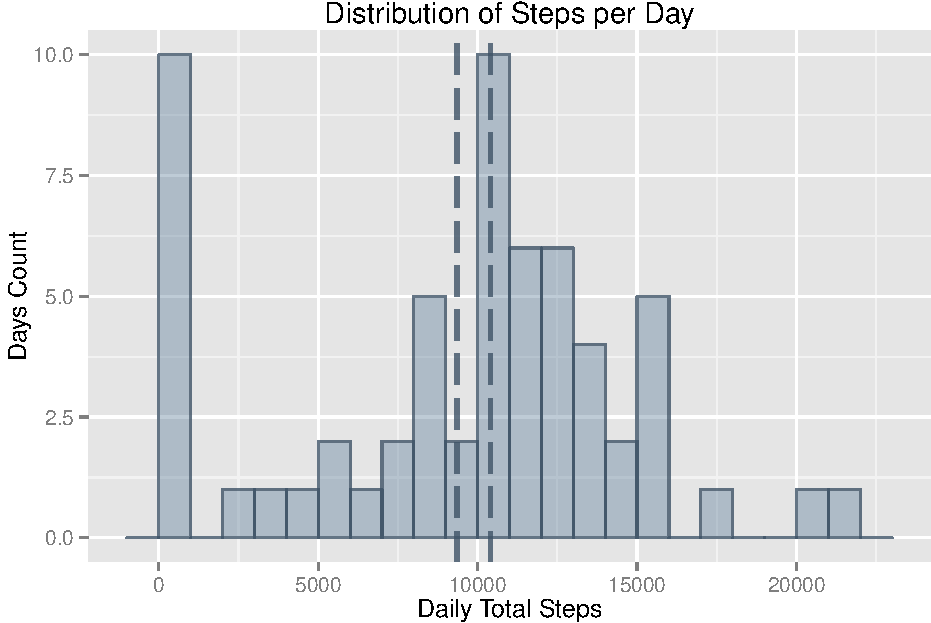
\includegraphics{PA1_template_files/figure-latex/unnamed-chunk-1-1.pdf}

\textbf{9354} is the \textbf{mean} number of steps taken in a day, as
calculated from data where NA is treated like no steps in that time
period

\textbf{10395} is the \textbf{median}, using the same data

\subsection{What is the average daily activity
pattern?}\label{what-is-the-average-daily-activity-pattern}

Calculate typical daily pattern, with NAs ignored and with NAs treated
as zero.

\begin{Shaded}
\begin{Highlighting}[]
\NormalTok{dailyPattern <-}\StringTok{ }\NormalTok{activity %>%}
\StringTok{    }\KeywordTok{group_by}\NormalTok{(time) %>%}\StringTok{ }
\StringTok{    }\KeywordTok{summarise}\NormalTok{(}\DataTypeTok{stepsZeroNAs=}\KeywordTok{mean}\NormalTok{(stepsZeroNAs), }
              \DataTypeTok{stepsTypical=}\KeywordTok{mean}\NormalTok{(steps, }\DataTypeTok{na.rm =} \OtherTok{TRUE}\NormalTok{))}
\KeywordTok{setkey}\NormalTok{(dailyPattern, time)}
\end{Highlighting}
\end{Shaded}

Then plot the data

\begin{Shaded}
\begin{Highlighting}[]
\KeywordTok{qplot}\NormalTok{(}\DataTypeTok{data =} \NormalTok{dailyPattern, }\DataTypeTok{y=}\NormalTok{stepsZeroNAs, }\DataTypeTok{x=}\NormalTok{time/}\DecValTok{3600}\NormalTok{, }\DataTypeTok{geom=}\StringTok{"line"}\NormalTok{, }
      \DataTypeTok{xlim =} \KeywordTok{c}\NormalTok{(}\DecValTok{0}\NormalTok{, }\DecValTok{24}\NormalTok{), }\DataTypeTok{xlab=}\StringTok{"Time Interval (hour)"}\NormalTok{, }\DataTypeTok{ylab=}\StringTok{"Steps"}\NormalTok{, }
      \DataTypeTok{main=}\StringTok{"Daily Pattern without Imputed Data"}\NormalTok{)}
\end{Highlighting}
\end{Shaded}

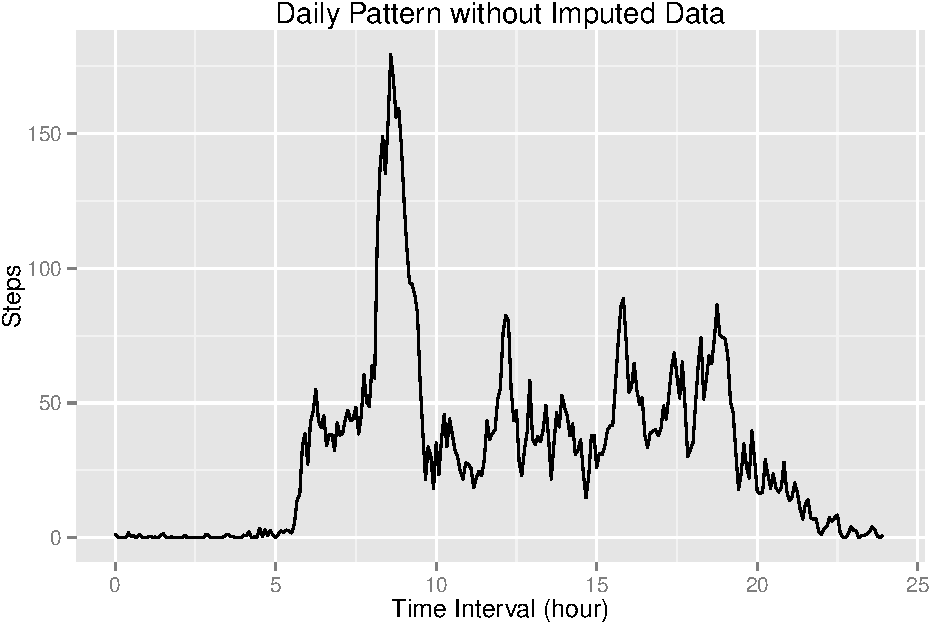
\includegraphics{PA1_template_files/figure-latex/unnamed-chunk-2-1.pdf}

From this calculation, we can note that typically, the most active
5-minute interval during the day starts at:

\begin{Shaded}
\begin{Highlighting}[]
\NormalTok{dailyPattern[stepsZeroNAs==}\KeywordTok{max}\NormalTok{(dailyPattern$stepsZeroNAs), time]}
\end{Highlighting}
\end{Shaded}

\begin{verbatim}
## [1] "08:35:00"
\end{verbatim}

\subsection{Imputing missing values}\label{imputing-missing-values}

The original data set contained \textbf{\texttt{2304}} NAs, out of a
total \textbf{\texttt{17568}} observations.

The typical number of steps at each time interval during the day was
calculated in the previous section

\begin{verbatim}
dailyPattern <- activity %>%
    group_by(time) %>% 
    summarise(stepsZeroNAs=mean(stepsZeroNAs), 
              stepsTypical=mean(steps, na.rm = TRUE))
\end{verbatim}

This table can be used to impute typical values for the NAs in the
original data set. It covers all time intervals during the day covered
by the earlier method of turing NAs into zeroes:

\begin{Shaded}
\begin{Highlighting}[]
\KeywordTok{length}\NormalTok{(}\KeywordTok{unique}\NormalTok{(dailyPattern$stepsTypical)) ==}\StringTok{ }\KeywordTok{length}\NormalTok{(}\KeywordTok{unique}\NormalTok{(dailyPattern$stepsZeroNAs))}
\end{Highlighting}
\end{Shaded}

\begin{verbatim}
## [1] TRUE
\end{verbatim}

And, it contains no NAs:

\begin{Shaded}
\begin{Highlighting}[]
\KeywordTok{sum}\NormalTok{(}\KeywordTok{is.na}\NormalTok{(}\KeywordTok{length}\NormalTok{(}\KeywordTok{unique}\NormalTok{(dailyPattern$stepsTypical))))}
\end{Highlighting}
\end{Shaded}

\begin{verbatim}
## [1] 0
\end{verbatim}

This table can be used to create a new column in the original data set
that imputes missing values from the typical daily pattern in cases
there were NA values previously.

\begin{Shaded}
\begin{Highlighting}[]
\NormalTok{activity <-}\StringTok{ }\NormalTok{activity %>%}\StringTok{ }
\StringTok{    }\KeywordTok{mutate}\NormalTok{(}\DataTypeTok{stepsTypical =} \KeywordTok{ifelse}\NormalTok{(}
        \DataTypeTok{test =} \KeywordTok{is.na}\NormalTok{(steps), }
        \DataTypeTok{yes =} \NormalTok{dailyPattern[time==time, stepsTypical],}
        \DataTypeTok{no =} \NormalTok{steps))}
\end{Highlighting}
\end{Shaded}

These new data can be plotted like before:

\begin{Shaded}
\begin{Highlighting}[]
\CommentTok{# add imputed data}
\NormalTok{stepCounts <-}\StringTok{ }\NormalTok{activity %>%}\StringTok{ }
\StringTok{    }\KeywordTok{group_by}\NormalTok{(date) %>%}\StringTok{ }
\StringTok{    }\KeywordTok{summarise}\NormalTok{(}\DataTypeTok{stepsZeroNAs=}\KeywordTok{sum}\NormalTok{(stepsZeroNAs),}
              \DataTypeTok{stepsImputed=}\KeywordTok{sum}\NormalTok{(stepsTypical)) }

\CommentTok{# mean and median}
\NormalTok{meanstepsImputed <-}\StringTok{ }\KeywordTok{mean}\NormalTok{(stepCounts$stepsImputed)}
\NormalTok{medianstepsImputed <-}\StringTok{ }\KeywordTok{median}\NormalTok{(stepCounts$stepsImputed) }

\CommentTok{# new colors}
\NormalTok{tempHue <-}\StringTok{ }\FloatTok{0.88}
    \NormalTok{ColB.light <-}\StringTok{ }\KeywordTok{hsv}\NormalTok{(}\DataTypeTok{h =} \NormalTok{tempHue, }\DataTypeTok{s =} \FloatTok{0.4}\NormalTok{, }\DataTypeTok{v =} \FloatTok{0.6}\NormalTok{, }\DataTypeTok{alpha =} \FloatTok{0.4}\NormalTok{)}
    \NormalTok{ColB.dark <-}\StringTok{ }\KeywordTok{hsv}\NormalTok{(}\DataTypeTok{h =} \NormalTok{tempHue, }\DataTypeTok{s =} \FloatTok{0.4}\NormalTok{, }\DataTypeTok{v =} \FloatTok{0.4}\NormalTok{, }\DataTypeTok{alpha =} \FloatTok{0.8}\NormalTok{)}

\CommentTok{# build the plot}
\NormalTok{dailySteps.Imputed <-}\StringTok{ }
\StringTok{  }\CommentTok{# choose data}
\StringTok{  }\KeywordTok{ggplot}\NormalTok{(}\DataTypeTok{data =} \NormalTok{stepCounts) +}
\StringTok{  }\CommentTok{# aesthetics, one series => histogram}
\StringTok{  }\KeywordTok{aes}\NormalTok{(}\DataTypeTok{x =} \NormalTok{stepsImputed) +}
\StringTok{  }\CommentTok{# geometric details of histogram, including coloring}
\StringTok{  }\KeywordTok{geom_histogram}\NormalTok{(}\DataTypeTok{fill=}\NormalTok{ColB.light, }\DataTypeTok{colour=}\NormalTok{ColB.dark, }\DataTypeTok{binwidth =} \DecValTok{1000}\NormalTok{) +}
\StringTok{  }\CommentTok{# annotate mean and median values}
\StringTok{  }\KeywordTok{geom_vline}\NormalTok{(}\DataTypeTok{xintercept=}\NormalTok{meanstepsImputed, }\DataTypeTok{colour=}\NormalTok{ColB.dark, }\DataTypeTok{size=}\FloatTok{1.0}\NormalTok{, }\DataTypeTok{linetype=}\StringTok{"longdash"}\NormalTok{) +}
\StringTok{  }\KeywordTok{geom_vline}\NormalTok{(}\DataTypeTok{xintercept=}\NormalTok{medianstepsImputed, }\DataTypeTok{colour=}\NormalTok{ColB.dark, }\DataTypeTok{size=}\FloatTok{1.0}\NormalTok{, }\DataTypeTok{linetype=}\StringTok{"longdash"}\NormalTok{) +}
\StringTok{  }\CommentTok{# Add labels}
\StringTok{  }\KeywordTok{labs}\NormalTok{(}
    \DataTypeTok{title =} \StringTok{"Distribution of Steps per Day (With Imputed Data)"}\NormalTok{, }
    \DataTypeTok{x =} \StringTok{"Daily Total Steps"}\NormalTok{, }\DataTypeTok{y =} \StringTok{"Days Count"}\NormalTok{)}

\CommentTok{# execute the plot}
\NormalTok{dailySteps.Imputed}
\end{Highlighting}
\end{Shaded}

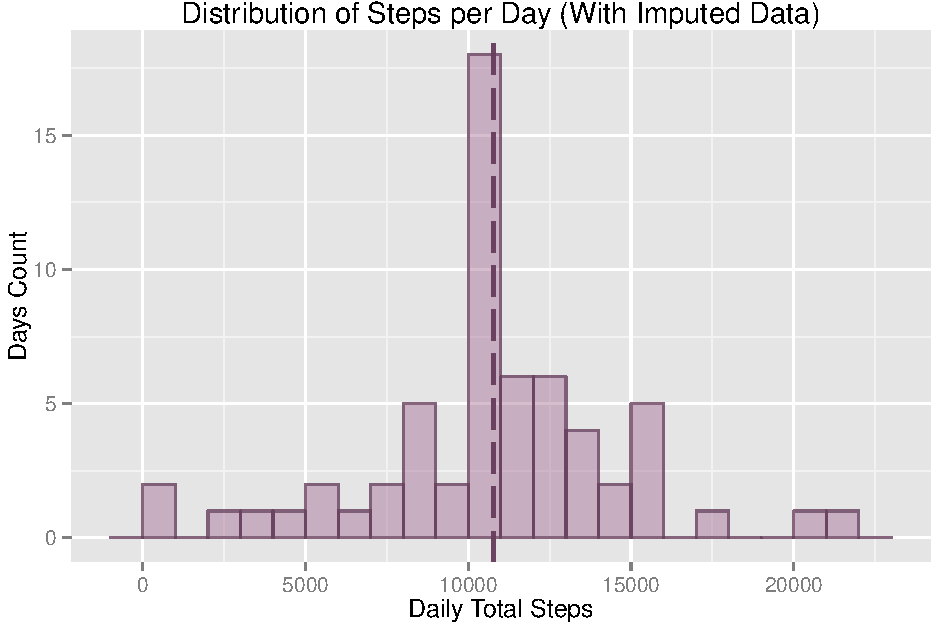
\includegraphics{PA1_template_files/figure-latex/unnamed-chunk-5-1.pdf}

\subsection{Are there differences in activity patterns between weekdays
and
weekends?}\label{are-there-differences-in-activity-patterns-between-weekdays-and-weekends}

\begin{Shaded}
\begin{Highlighting}[]
\NormalTok{activity <-}\StringTok{ }\NormalTok{activity %>%}
\StringTok{  }\KeywordTok{mutate}\NormalTok{(}\DataTypeTok{weekday=} \KeywordTok{ifelse}\NormalTok{(}
    \KeywordTok{weekdays}\NormalTok{(date) %in%}\StringTok{ }\KeywordTok{c}\NormalTok{(}\StringTok{"Saturday"}\NormalTok{, }\StringTok{"Sunday"}\NormalTok{), }
    \StringTok{"Weekend"}\NormalTok{, }
    \StringTok{"Weekday"}\NormalTok{))}

\NormalTok{dailyPattern.split <-}\StringTok{ }\NormalTok{activity %>%}
\StringTok{    }\KeywordTok{group_by}\NormalTok{(time, weekday) %>%}
\StringTok{    }\KeywordTok{summarise}\NormalTok{(time, }\DataTypeTok{steps=}\KeywordTok{mean}\NormalTok{(stepsTypical))}

\KeywordTok{ggplot}\NormalTok{(}\DataTypeTok{data =} \NormalTok{dailyPattern.split, }\KeywordTok{aes}\NormalTok{(}\DataTypeTok{x =} \KeywordTok{as.POSIXct}\NormalTok{(time), }\DataTypeTok{y =} \NormalTok{steps, }\DataTypeTok{color =} \NormalTok{weekday)) +}\StringTok{ }
\StringTok{  }\KeywordTok{scale_x_datetime}\NormalTok{(}\DataTypeTok{breaks =} \KeywordTok{date_breaks}\NormalTok{(}\StringTok{"2 hour"}\NormalTok{), }\DataTypeTok{labels =} \KeywordTok{date_format}\NormalTok{(}\StringTok{"%l %p"}\NormalTok{)) +}
\StringTok{  }\CommentTok{# See documentation for `scales` package to understand `scale_x_datetime`,}
\StringTok{  }\CommentTok{# `date_breaks` and `date_format` transformation of times along x-axis}
\StringTok{  }\KeywordTok{facet_grid}\NormalTok{(weekday ~}\StringTok{ }\NormalTok{.) +}\StringTok{ }\KeywordTok{geom_line}\NormalTok{() +}\StringTok{ }
\StringTok{  }\KeywordTok{labs}\NormalTok{(}\DataTypeTok{title =} \KeywordTok{sprintf}\NormalTok{(}
    \StringTok{"Distribution of Steps Taken }\CharTok{\textbackslash{}n}\StringTok{by Time of Day }\CharTok{\textbackslash{}n}\StringTok{Weekend vs. Weekdays"}\NormalTok{), }
    \DataTypeTok{x =} \StringTok{"Interval"}\NormalTok{, }\DataTypeTok{y =} \StringTok{"Steps per 5-minute Interval"}\NormalTok{)}
\end{Highlighting}
\end{Shaded}

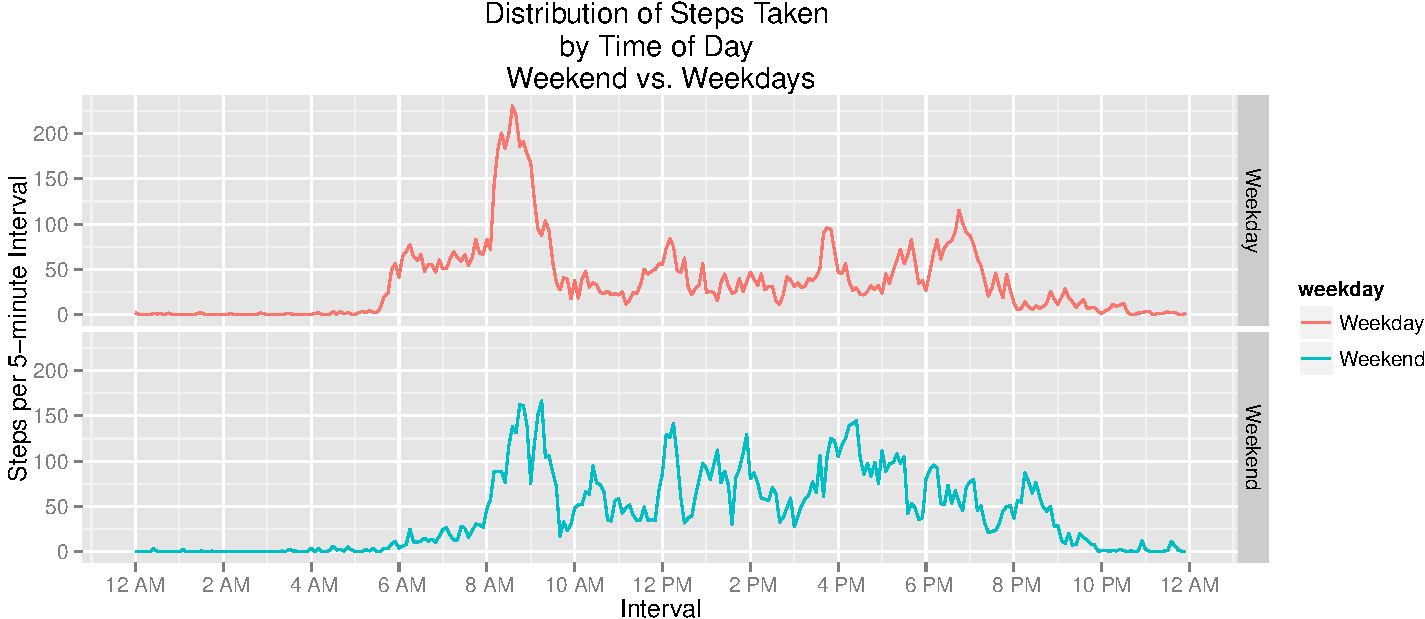
\includegraphics{PA1_template_files/figure-latex/unnamed-chunk-6-1.pdf}

And, just for fun here is an additional plot of the data

\begin{Shaded}
\begin{Highlighting}[]
\KeywordTok{ggplot}\NormalTok{(}\DataTypeTok{data =} \NormalTok{activity, }\KeywordTok{aes}\NormalTok{(}\DataTypeTok{x =} \KeywordTok{as.POSIXct}\NormalTok{(time), }\DataTypeTok{y =} \NormalTok{stepsTypical, }\DataTypeTok{colour =} \NormalTok{weekday, }\DataTypeTok{fill =} \NormalTok{weekday)) +}\StringTok{ }
\StringTok{  }\KeywordTok{scale_x_datetime}\NormalTok{(}\DataTypeTok{breaks =} \KeywordTok{date_breaks}\NormalTok{(}\StringTok{"2 hour"}\NormalTok{), }\DataTypeTok{labels =} \KeywordTok{date_format}\NormalTok{(}\StringTok{"%l %p"}\NormalTok{)) +}\StringTok{ }
\StringTok{  }\KeywordTok{stat_smooth}\NormalTok{(}\DataTypeTok{method =} \StringTok{"gam"}\NormalTok{) +}\StringTok{  }\KeywordTok{geom_smooth}\NormalTok{(}\DataTypeTok{level =} \FloatTok{0.8}\NormalTok{) +}\StringTok{ }
\StringTok{  }\KeywordTok{geom_point}\NormalTok{(}\DataTypeTok{alpha=}\FloatTok{0.5}\NormalTok{, }\DataTypeTok{size=}\DecValTok{1}\NormalTok{, }\DataTypeTok{position =} \StringTok{"jitter"}\NormalTok{) +}
\StringTok{  }\KeywordTok{labs}\NormalTok{(}\DataTypeTok{title =} \KeywordTok{sprintf}\NormalTok{(}
    \StringTok{"Distribution of Steps Taken }\CharTok{\textbackslash{}n}\StringTok{by Time of Day }\CharTok{\textbackslash{}n}\StringTok{Weekend vs. Weekdays"}\NormalTok{), }
    \DataTypeTok{x =} \StringTok{"Time of Day"}\NormalTok{, }\DataTypeTok{y =} \StringTok{"Steps per 5-minute Interval"}\NormalTok{)}
\end{Highlighting}
\end{Shaded}

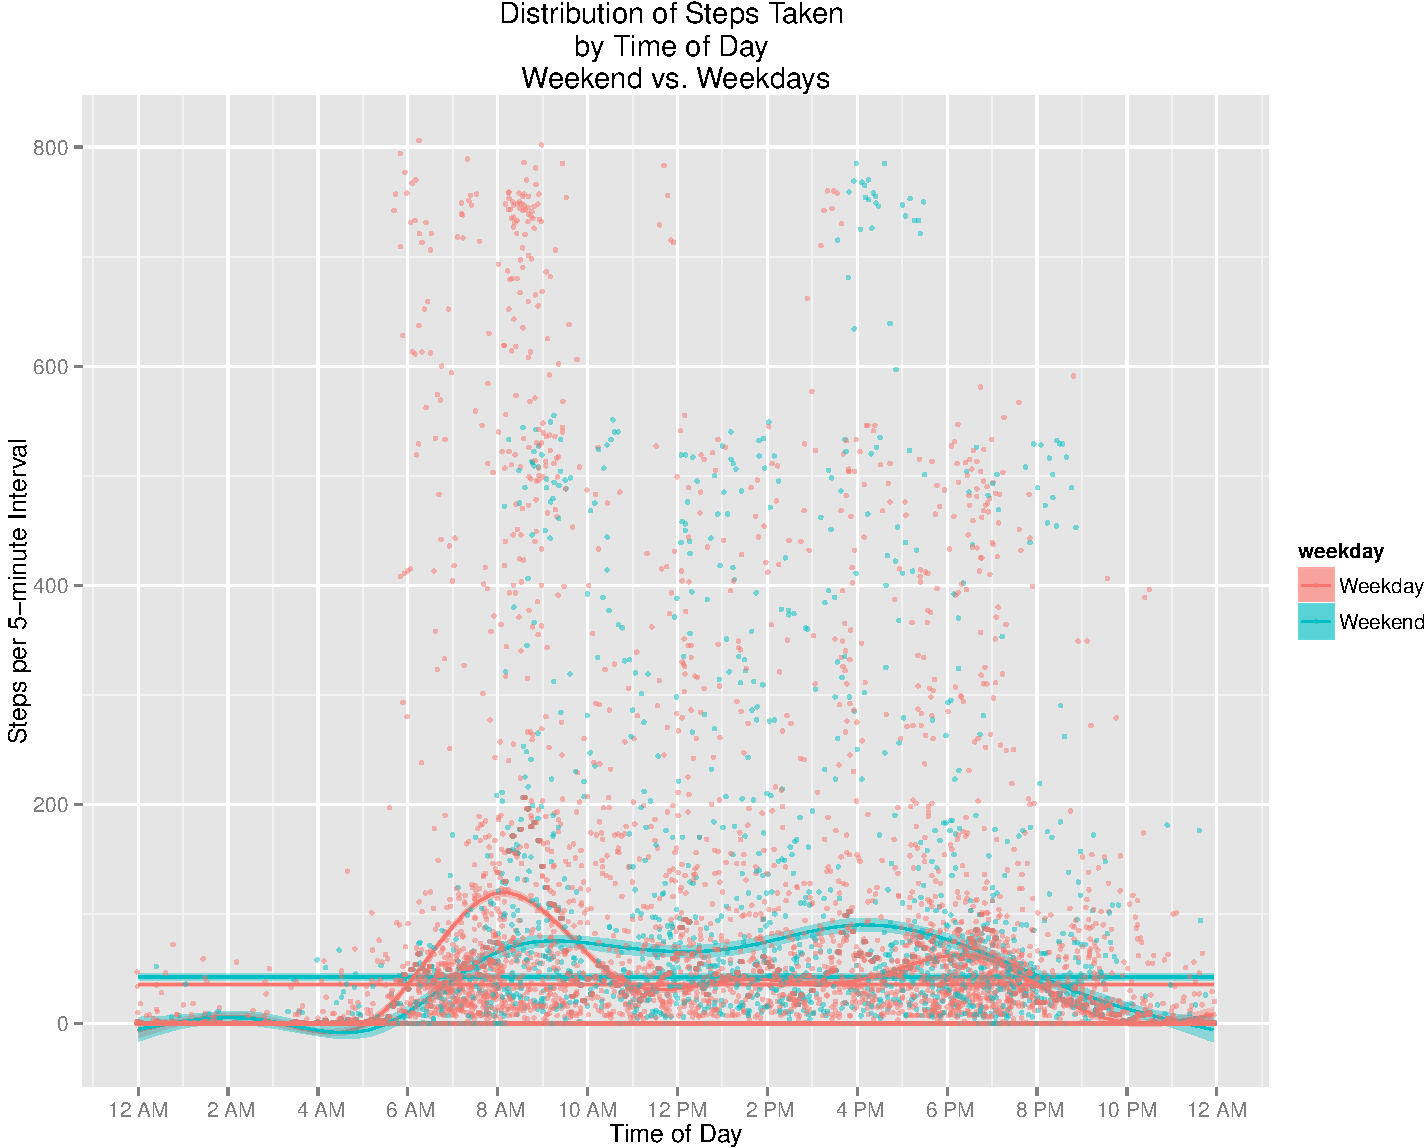
\includegraphics{PA1_template_files/figure-latex/unnamed-chunk-7-1.pdf}

And, zooming in on the smoothed data

\begin{Shaded}
\begin{Highlighting}[]
\KeywordTok{ggplot}\NormalTok{(}\DataTypeTok{data =} \NormalTok{activity, }
       \KeywordTok{aes}\NormalTok{(}\DataTypeTok{x =} \KeywordTok{as.POSIXct}\NormalTok{(time), }\DataTypeTok{y =} \NormalTok{stepsTypical, }\DataTypeTok{colour =} \NormalTok{weekday, }\DataTypeTok{fill =} \NormalTok{weekday)) +}\StringTok{ }
\StringTok{  }\KeywordTok{scale_x_datetime}\NormalTok{(}\DataTypeTok{breaks =} \KeywordTok{date_breaks}\NormalTok{(}\StringTok{"2 hour"}\NormalTok{), }\DataTypeTok{labels =} \KeywordTok{date_format}\NormalTok{(}\StringTok{"%l %p"}\NormalTok{)) +}
\StringTok{  }\KeywordTok{stat_smooth}\NormalTok{(}\DataTypeTok{method =} \StringTok{"gam"}\NormalTok{) +}\StringTok{  }\KeywordTok{geom_smooth}\NormalTok{(}\DataTypeTok{level =} \FloatTok{0.6}\NormalTok{) +}
\StringTok{  }\KeywordTok{labs}\NormalTok{(}\DataTypeTok{title =} \KeywordTok{sprintf}\NormalTok{(}\StringTok{"Distribution of Steps Taken }\CharTok{\textbackslash{}n}\StringTok{by Time of Day }\CharTok{\textbackslash{}n}\StringTok{Weekend vs. Weekdays"}\NormalTok{), }
       \DataTypeTok{x =} \StringTok{"Time of Day"}\NormalTok{, }\DataTypeTok{y =} \StringTok{"Steps per 5-minute Interval"}\NormalTok{)}
\end{Highlighting}
\end{Shaded}

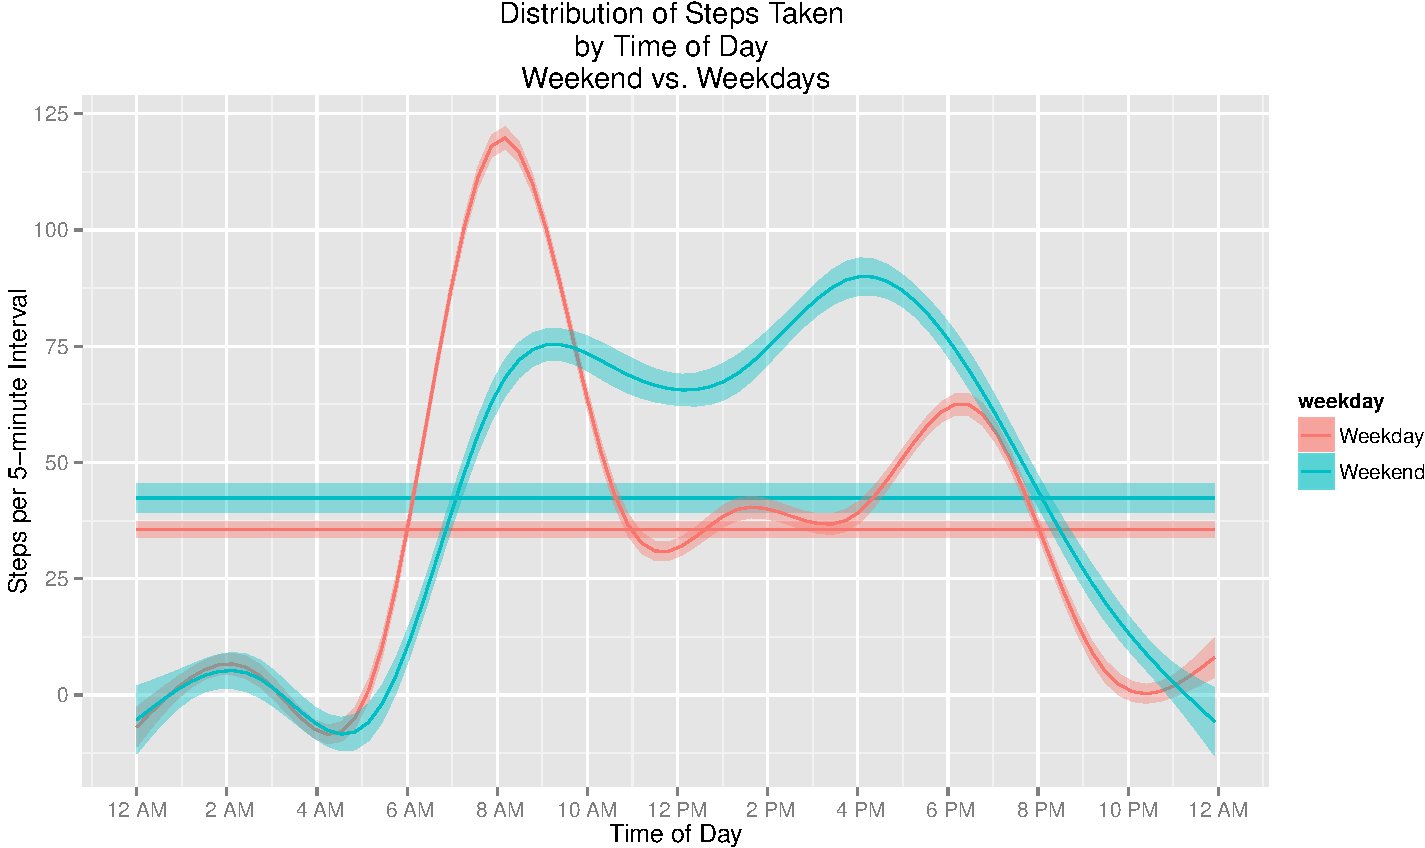
\includegraphics{PA1_template_files/figure-latex/unnamed-chunk-8-1.pdf}

\subsection{Appendix A: Environment}\label{appendix-a-environment}

\begin{Shaded}
\begin{Highlighting}[]
\KeywordTok{sessionInfo}\NormalTok{()}
\end{Highlighting}
\end{Shaded}

\begin{verbatim}
## R version 3.1.2 (2014-10-31)
## Platform: x86_64-apple-darwin13.4.0 (64-bit)
## 
## locale:
## [1] en_US.UTF-8/en_US.UTF-8/en_US.UTF-8/C/en_US.UTF-8/en_US.UTF-8
## 
## attached base packages:
## [1] stats     graphics  grDevices utils     datasets  methods   base     
## 
## other attached packages:
## [1] mgcv_1.8-4       nlme_3.1-119     scales_0.2.4     ggplot2_1.0.0   
## [5] dplyr_0.4.1      data.table_1.9.4
## 
## loaded via a namespace (and not attached):
##  [1] assertthat_0.1   chron_2.3-45     colorspace_1.2-4 DBI_0.3.1       
##  [5] digest_0.6.8     evaluate_0.5.5   formatR_1.0      grid_3.1.2      
##  [9] gtable_0.1.2     htmltools_0.2.6  knitr_1.8        labeling_0.3    
## [13] lattice_0.20-29  lazyeval_0.1.10  magrittr_1.5     MASS_7.3-37     
## [17] Matrix_1.1-4     munsell_0.4.2    parallel_3.1.2   plyr_1.8.1      
## [21] proto_0.3-10     Rcpp_0.11.3      reshape2_1.4.1   rmarkdown_0.4.2 
## [25] stringr_0.6.2    tools_3.1.2      yaml_2.1.13
\end{verbatim}

\subsection{Appendix B: Notes on Selected R
Packages}\label{appendix-b-notes-on-selected-r-packages}

\subsubsection{dplyr 0.4.1}\label{dplyr-0.4.1}

\begin{itemize}
\itemsep1pt\parskip0pt\parsep0pt
\item
  summary \url{https://github.com/hadley/dplyr/blob/v0.4.1/README.md}
\item
  news \url{https://github.com/hadley/dplyr/blob/v0.4.1/NEWS.md}
\end{itemize}

\textbf{Dplyr} by Hadley Wickam builds upon the earlier \texttt{plyr}
package for data manipulation and shaping for analysis. Execution speed
approaches that of \texttt{data.table} with syntax patterns that are
arguabley more consistent with other R packages. Additionally,
\texttt{dplyr} can serve as a wrapper around \texttt{data.table}
objects.

Note that \texttt{dplyr} also automatically imports \texttt{magrittr}

\begin{itemize}
\item
  \texttt{mutate()} - This function takes a data.frame or data.table in
  dplyr and adds columns with values as specified. It leaves existing
  columns in place regardless of whether they are specified. This is in
  contrast to \texttt{transmute()} which drops any existing columns that
  are not specified to be output.
\item
  \texttt{group\_by()} \& \texttt{summarise()} - Replicate functinality
  found in base R functions like \texttt{aggregate()},
  \texttt{*apply()}, \texttt{by()} and \texttt{subset()}
\end{itemize}

\subsubsection{magrittr 1.5}\label{magrittr-1.5}

\begin{itemize}
\itemsep1pt\parskip0pt\parsep0pt
\item
  overview
  \url{https://github.com/smbache/magrittr/blob/v.1.5/README.md}
\item
  vignettes
  \url{http://cran.r-project.org/web/packages/magrittr/vignettes/magrittr.html}
\end{itemize}

\textbf{Magrittr} supplies a ``forward pipe'' operator
\texttt{\%\textgreater{}\%} which is useful for composing functions. The
following two expressions:

\begin{verbatim}
order(upper(c("c", "b", "a")))
\end{verbatim}

is equivalent to:

\begin{verbatim}
c("c", "b", "a") %>%
    upper() %>%
    order()
\end{verbatim}

\subsubsection{scales 0.2.4}\label{scales-0.2.4}

Required for ggplot2's \texttt{scale\_x\_dateime}
\url{http://docs.ggplot2.org/current/scale_datetime.html}

\subsubsection{tidyr 0.2.0}\label{tidyr-0.2.0}

\begin{itemize}
\itemsep1pt\parskip0pt\parsep0pt
\item
  summary \url{https://github.com/hadley/tidyr/blob/v0.2.0/README.md}
\item
  source \url{https://github.com/hadley/tidyr}
\item
  CRAN \url{http://cran.r-project.org/web/packages/tidyr/index.html}
\end{itemize}

\textbf{Tidyr} can be used to shape data. In database theory, such
operation are equivalent to changing between different normal forms.
Tidyr focuses around \texttt{gather()}, which makes wide tables tall,
and \texttt{spread()} which makes tall tables wide.

\end{document}
